% -----------------------------------------------
%   GeoTracking Block
% -----------------------------------------------
\subsection{Geo-tracking Block}
We enabled per-bundle tracking by defining the {\em GeoTracking} extension block, which, when attached to any bundle, collects both the logical hops that the bundle traverses and the bundle's trajectory through physical space. The {\em GeoTracking} block is a series of tracking entries (each one either recording a logical hop or a physical location) prefaced by a small header containing parameters for maintaining the block and counting the number of its entries.
\begin{figure}
\begin{center}
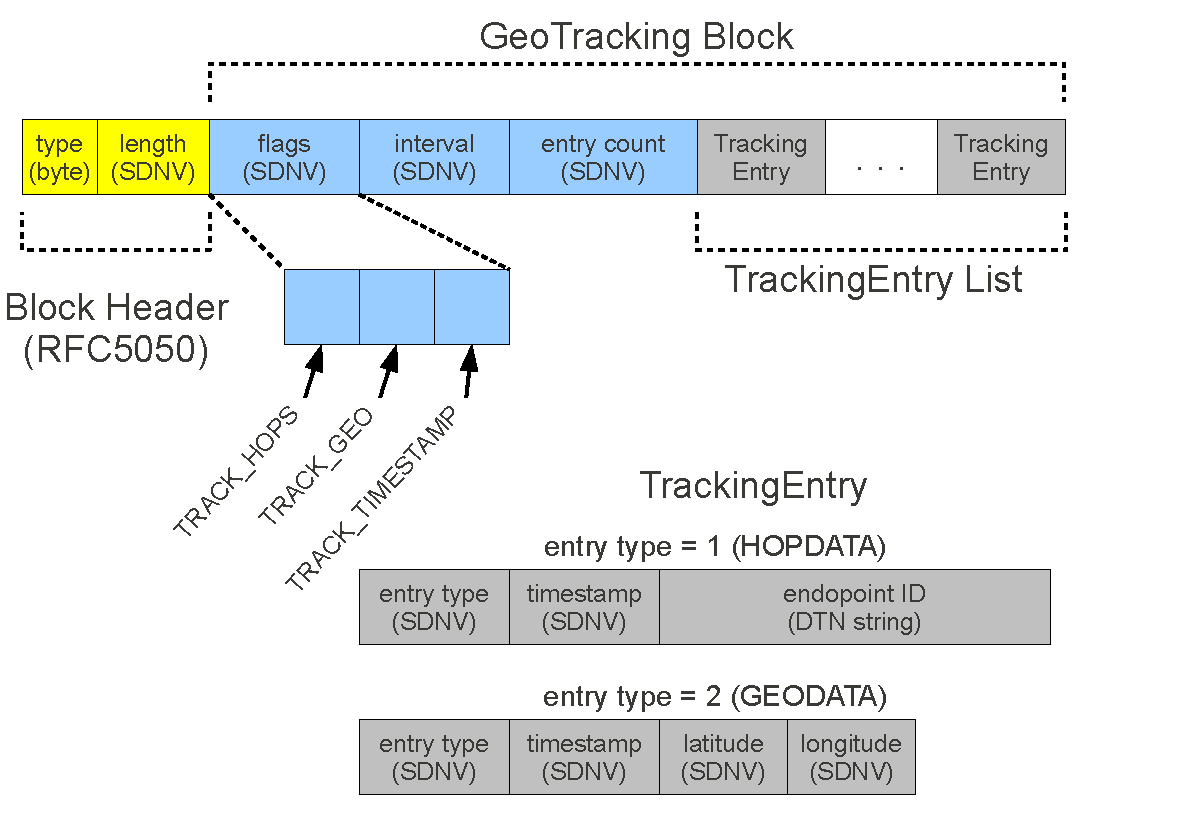
\includegraphics[width=\columnwidth]{figures/tracking-block.pdf}
\end{center}
\caption{Format of the GeoTracking Block}
\label{fig:tracking-block}
\end{figure}

\begin{sloppypar}
Figure~\ref{fig:tracking-block} depicts the {\em GeoTracking} block's format. The Block Header fields are specified by RFC5050\footnote{\url{http://tools.ietf.org/html/rfc5050}} and apply to any block in a bundle. In IBR-DTN, the block processor only deals with the contents of the block itself, and the BPA strips off the block header. Each {\em GeoTracking} block contains three mandatory fields:
\begin{description*}
  \item[Flags.] The flags tell intermediate BPAs what information to append to the block. The flags are: {\bf TRACK\_HOPS} (0x01), {\bf TRACK\_GEO} (0x02), and {\bf TRACK\_TIMESTAMP} (0x04).
  \item[Interval.] The interval (in seconds) tells intermediate BPAs the frequence with which to append a new GEODATA tracking entry to the entry list.  
  \item[Entry Count.] The entry count keeps track of the number of tracking entries contained in the block.
\end{description*}
\end{sloppypar}

Maintaining and updating the GeoTracking block is a dilemma.  We would like for the block stored in the BPA to always be up to date, but it is not feasible to update it in real time for several reasons.  First, the may be many bundles held at the BPA with GeoTracking blocks, and with tracking specified at different intervals.  Updating them all in real time would require quite a few timers, and (in the case of IBR-DTN) reloading/storing each of those bundles from disk each time a new entry is to be attached.  We concluded that it is best to maintain a global GPS log and to only update the GeoTracking block when a bundle is serialized for sending.  The maintainence of this global GPS log then becomes an issue.  In order to completely satisfy the tracking interval requirements of each bundle with a GeoTracking block we would need it to record the node's location at an interval of the GCD of all the tracking intervals.  In our prototype we choose a fixed global interval appropriate to the experiment and bundles can request a {\it less frequent} update.  Finally there is the question of where the GPS log should be maintained.  It could concievably be maintained in the BPA itself, however access to GPS information is a very platform-specific process, whereas a good BPA should be portable.  Also it would require an extra timer or thread in the BPA for a fairly specialized feature.  Our solution is to have a host-specific agent that logs GPS data to a file at an interval chosen by the host.  Each time a GeoTracking block is to be serialized the BPA scans this file for the desired entries and creates the necessary TrackingEntry fields for the Tracking Block.

This method of maintaining GPS data still has some drawbacks, especially in IBRDTN.  First, it requires opening and reading a (potentially long) log file each time a Geotracking block is serialized.  Second, in IBRDTN, because there is no function to "finalize" the contents of a block prior to serializing, the GPS log must be parsed twice.  Once when the block processor calculates the block's length, and again when the actual serialization takes place.  In IBRDTN both the {\bf getLength()} and {\bf serialize()} functions are {\bf const}, so it is not possible to modify any fields of the GeoTracking block itself to cache the state of the block when {\bf getLength()} is called.  This techniclaly creates a race condition between these two calls, where the GPS log may get longer between when {\bf getLength()} and {\bf serialize()} are called.  Resolving these issues completely may require some modifications to the serialization process of IBR-DTN and is reserved for future work (for Johannes).

\subsubsection{GPS Coordinate Representation as SDNV} \label{gps-representation}
Our extension blocks represent GPS coordinates in signed degrees format, where latitude ranges from $-90^{\circ}$ to $90^{\circ}$ and longitude ranges from $-180^{\circ}$ to $180^{\circ}$.  Both latitude and longitude are considered to be type {\bf float}.  However since SDNVs cannot represent floating point numbers or negative integers we make two transformations to encode them in the block.  If $\theta<0$ we compute $\theta^{\prime}=\theta+360^{\circ}$.  Then we scale all coordinates up by a factor of $1048576$.  This gives us at least 20 bits of precision in both values; more than enough for meter-level resoloution in the GPS coordinates.  When the blocks are received and deserialized these transforms are reversed to give the original floating point lat/lon values.



